\documentclass{report}
\usepackage[margin=1in, paperwidth=8.5in, paperheight=11in]{geometry}
%Math packages%
\usepackage{amsmath}
\usepackage{amsthm}
%Spacing%
\usepackage{setspace}
\onehalfspacing
%Lecture number%
\newcommand{\lectureNum}{7}
%Variables - Date and Course%
\newcommand{\curDate}{March 2, 2017}
\newcommand{\course}{CS 251}
\newcommand{\instructor}{Stephen Mann}
%Defining the example tag%
%\theoremstyle{definition}%
\newtheorem{ex}{Example}[section]
%Setting counter given the lecture number%
\setcounter{chapter}{\lectureNum{}}
%Package to insert code%
\usepackage{listings}
\usepackage{courier}
\usepackage{xcolor}
\lstset { %
    tabsize=2,
    breaklines=true,
    language=C++,
    backgroundcolor=\color{blue!8}, % set backgroundcolor
    basicstyle=\footnotesize\ttfamily,% basic font setting
}
%Package used to draw circuits%
\usepackage{circuitikz}
\begin{document}
%Note title%
\begin{center}
\begin{Large}
\textsc{\course{} | Chapter \lectureNum{}: Memory Hierarchy}
\end{Large}
\end{center} 
\noindent \textit{Bartosz Antczak} \hfill
\textit{Instructor: \instructor{}} \hfill
\textit{\curDate{}}
\rule{\textwidth}{0.4pt}
% Actual Notes%
\section{Introduction}
\subsubsection{Key Questions}
\begin{itemize}
\item What is memory hierarchy?
\item Why do we have them?
\end{itemize}
\subsubsection{Fast Memory}
When we say that memory is \textit{fast}, we say that the time required to access it is relatively fast. For instance, from figures in 2012:
\begin{itemize}
\item SRAM typically only requires 0.5 - 2.5 nanoseconds to access memory (costs \$500 - \$1,000)
\item A Magnetic Disk requires 5,000,000 - 7,000,000 nanoseconds (costs around 5 cents)
\end{itemize}
Obviously, the faster the memory, the more expensive it becomes.\\
The \textbf{goal} of memory hierarchies is to create an illusion of unlimited fast memory. This is done by having several types and sizes of memory, each of varying speed. We move items to smaller, faster memory automatically when they are needed, and we keep them there if they are used often.
The general hierarchy is structured (from the fastest being at the top):
\begin{itemize}
\item Registers
\item \textit{L1, L2, L3 caches} (which are small amounts of memory on the processor
\item RAM
\item Disk
\item Local network
\item The cloud / off site storage
\end{itemize}
\subsection{Implementation}
The items not in the top level are brought up when requested. They're not copied directly to the front, however. The data is only copied between adjacent levels (this is identical to the transpose heuristic outlined in CS 240).\\
Starting at the top of the hierarchy, we look for the data in each section of memory. If the data is not there, move down one level. If the data is found, retrieve it and swap this memory with the memory in the upper level.\\
This hierarchy sees memory as a \textbf{single array}.
\section{Implementing a Cache}
\subsubsection{Key Questions}
\begin{itemize}
\item How is a cache organized?
\item What are the basic challenges with caching?
\end{itemize}
Recall that cache is a small amount of memory in the processor. We have an L1, L2, and L3 cache:
\begin{itemize}
\item \textbf{L1:} 32 KB instruction, 32 KB data per core
\item \textbf{L2:} 256 KB per core
\item \textbf{L3:} 2-4 MB shared with all cores
\end{itemize}
\subsection{Approach 1: Direct Mapped Cache}
This approach requires that each memory location is mapped to exactly one location in the cache.
\subsubsection{Storing and Looking for Data}
Assume $M$ blocks of cache memory, where each block has size $B$. When given a request for address $p$, translate it into a request for cache block $m$ (if cache entry is valid). The typical mapping for a cache block is:
$$m = (p/B)\mod M$$
\begin{ex}
An example mapping for a cache
\end{ex}
\begin{figure}[ht]
\begin{center}
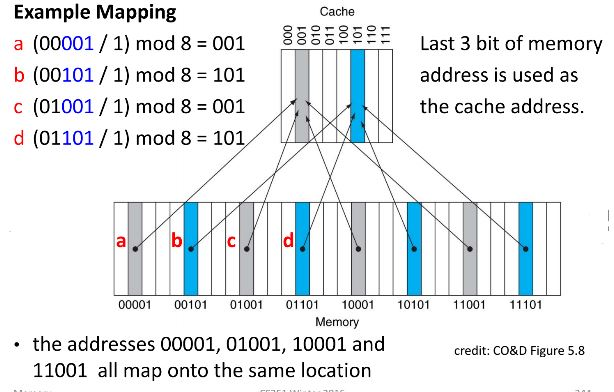
\includegraphics[scale=0.7]{direct_map1.jpg}
\end{center}
\caption{\textit{Courtesy of Kevin Lanctot's Winter 2016 slides}}
\end{figure}
\subsubsection{Tags}
Many memory blocks map to the same cache block. Adding \textbf{tags} will identify which memory block is actually present. For example (referring to the previous example), the tag would be the upper 2 bits. If the cache location 101 (called the index) contains the value of memory location 00\textbf{101}, then its tag will be 00 (the first two bits).
\subsubsection{Valid Bits}
We must track if the cache entry is valid. We do this by adding a valid bit.
\begin{ex}
Storing and looking for data in a cache
\end{ex}
\begin{center}
\textbf{Cache}\\
\begin{tabular}{ l | l | l | l }
\hline
Index & Valid & Tag & Data \\\hline
000 & N & & \\
001 & N & & \\
010 & Y & 11 & Mem[11010] \\
011 & N & & \\
100 & N & & \\
101 & N & & \\
110 & Y & 10 & Mem[10110] \\
111 & N & & \\
\end{tabular}
\end{center}
We perform these following instructions on the cache:
\begin{center}
\begin{tabular}{ c | c | c | c }
\hline Action & Word Address & Binary Address & Hit/Miss \\\hline
Load Word & 22 & 10 \textbf{110} & Miss \\
Load Word & 26 & 11 \textbf{010} & Miss \\
Load Word & 22 & 10 \textbf{110} & Hit (Does not alter cache) \\
Load Word & 26 & 11 \textbf{010} & Hit (Does not alter cache)\\
\end{tabular}
\end{center}
Now what if we loaded the following:
\begin{center}
\begin{tabular}{ c | c | c | c }
\hline Action & Word Address & Binary Address & Hit/Miss \\\hline
Load Word & 18 & 10 \textbf{010} & Miss \\
\end{tabular}
\end{center}
Here, we \textit{overwrite} whatever was in index 010 (which was Mem[\textit{11}010]) with Mem[\textit{10}010].
\subsubsection{What Happens on a Cache Miss?}
We stall the entire processor until the item has been fetched.
%END%
\end{document}